
%%%%%%%%%%%%%%%%%%%%%%%%%%%%%%%%%%%%%%%%%%%%%%%%%%%
\section{Toolkit - Components}
\label{sec:components}
%%%%%%%%%%%%%%%%%%%%%%%%%%%%%%%%%%%%%%%%%%%%%%%%%%%

Joining the algorithms and techniques described in the previous sections, we propose now the creation of a toolkit that would allow developers to create, implement, and expand the existing components. Figure \ref{fig:compdiag} shows a component diagram that represents the initial setup of the toolkit, and that provides the users with the choice to: 1) What \ac{ml} algorithm to use; 2) What privacy-preserving technique to use; 3) The dataset to process; and 4) Inspect the resulting data.

\begin{figure}[H]
  \centerline{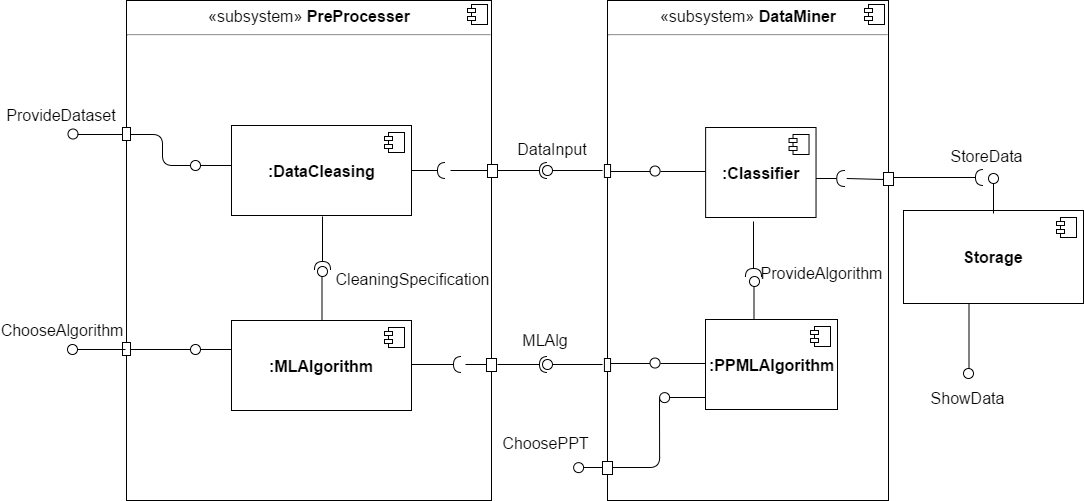
\includegraphics[width=1.1\textwidth]{images/CompDiagram.png}}
  \caption{Component Diagram for \acs{bard}.}
  \label{fig:compdiag}
\end{figure} 


Finally, we present now how \acs{bard} toolkit could be implemented in a business scenario. The users, in this case the companies that profit from using \ac{bard} to do knowledge learning, provide the dataset to train the model or select an existing model already trained with publicly available data, and provide the sample to be evaluated. A team of developers, that could be outsourced or part of the company, maintain the toolkit and develop new functionalities (new \ac{ml} algorithms, new privacy-preserving techniques, etc.). A central repository, that contains \ac{ml} models trained \textit{a priori} for different types of data context (healthcare, income, etc.). In figure \ref{fig:contextdiag}, we present a context diagram for \acs{bard}.


\begin{figure}[H]
  \centerline{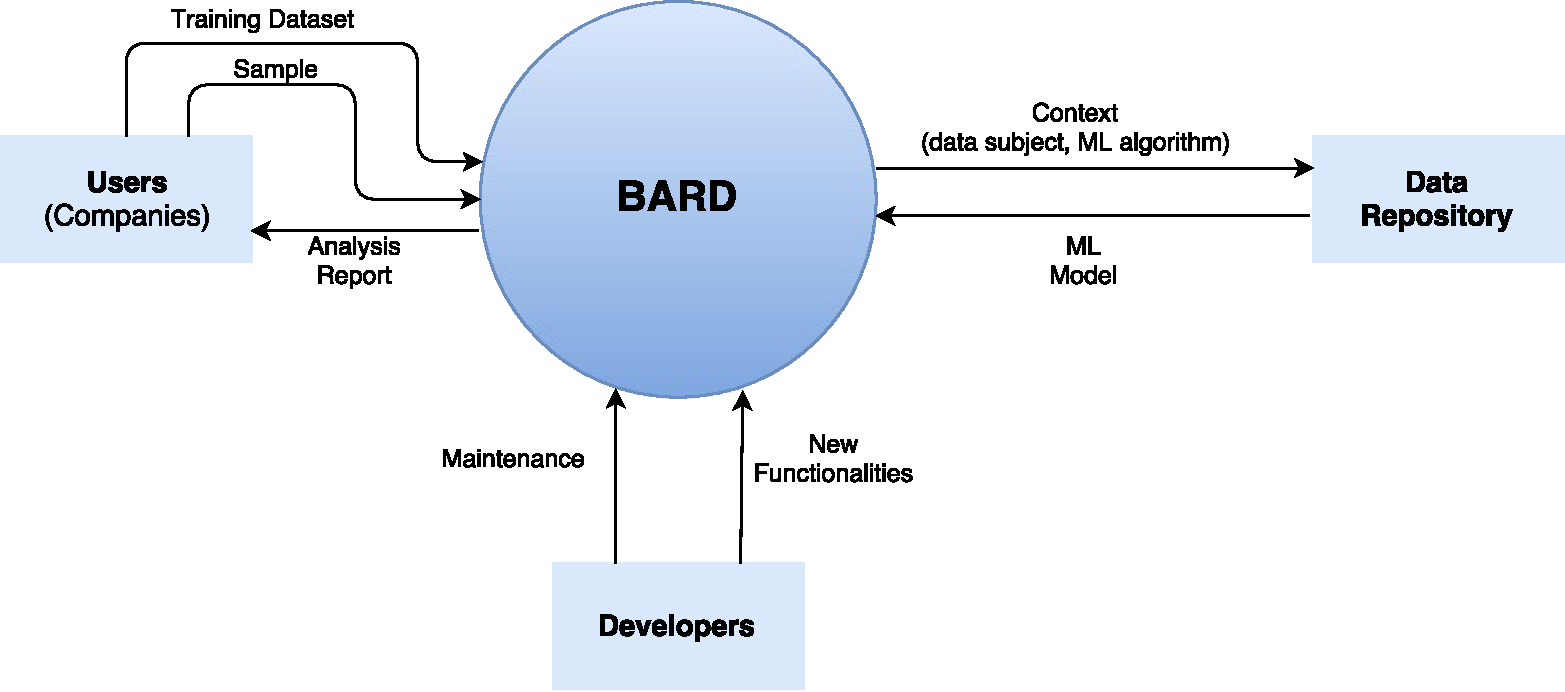
\includegraphics[width=1.1\textwidth]{images/ContextBard.pdf}}
  \caption{Context diagram for \acs{bard}.}
  \label{fig:contextdiag}
\end{figure} 